\documentclass[12pt]{article}
\usepackage[margin=2.5cm]{geometry}
\usepackage{enumerate}
\usepackage{amsfonts}
\usepackage{amsmath}
\usepackage{fancyhdr}
\usepackage{amsmath}
\usepackage{amssymb}
\usepackage{amsthm}
\usepackage{mdframed}
\usepackage{graphicx}
\usepackage{subcaption}
\usepackage{adjustbox}
\usepackage{listings}
\usepackage{xcolor}
\usepackage{booktabs}
\usepackage[utf]{kotex}
\usepackage{hyperref}
\usepackage{accents}

\definecolor{codegreen}{rgb}{0,0.6,0}
\definecolor{codegray}{rgb}{0.5,0.5,0.5}
\definecolor{codepurple}{rgb}{0.58,0,0.82}
\definecolor{backcolour}{rgb}{0.95,0.95,0.92}

\lstdefinestyle{mystyle}{
    backgroundcolor=\color{backcolour},
    commentstyle=\color{codegreen},
    keywordstyle=\color{magenta},
    numberstyle=\tiny\color{codegray},
    stringstyle=\color{codepurple},
    basicstyle=\ttfamily\footnotesize,
    breakatwhitespace=false,
    breaklines=true,
    captionpos=b,
    keepspaces=true,
    numbers=left,
    numbersep=5pt,
    showspaces=false,
    showstringspaces=false,
    showtabs=false,
    tabsize=1
}

\lstset{style=mystyle}

\pagestyle{fancy}
\renewcommand{\headrulewidth}{0.4pt}
\lhead{CSC 343}
\rhead{Worksheet 14}

\begin{document}
\title{CSC343 Worksheet 14}
\maketitle

\begin{enumerate}[1.]
    \item \textbf{Exercise 4.1.1:} Design a database for a bank, including information
    about customers and their accounts. Information about a customer includes their
    name, address, phone, and Social Security number. Accounts have numbers,
    types (e.g., savings, checking) and balances. Also record the customer(s) who
    own an account. Draw the E/R diagram for this database. Be sure to include
    arrows where appropriate, to indicate the multiplicity of a relationship.

    \item \textbf{Exercise 4.1.2:} Modify your solution to Exercise 4.1.1 as follows:

    \bigskip

    \begin{enumerate}[a)]
        \item Change your diagram so an account can have only one customer.
        \item Further change your diagram so a customer can have only one account.
        \item Change your original diagram of Exercise 4.1.1 so that a customer can have a set of addresses (which are street-city-state triples) and a set of phones. Remember that we do not allow attributes to have nonprimitive types, such as sets, in the E/R model.
        \item Further modify your diagram so that customers can have a set of addresses, and at each address there is a set of phones.
    \end{enumerate}

    \item \textbf{Exercise 4.1.3:} Give an E/R diagram for a database recording information
    about teams, players, and their fans, including:

    \begin{enumerate}[1.]
        \item For each team, its name, its players, its team captain (one of its players), and the colors of its uniform.
        \item For each player, his/her name.
        \item For each fan, his/her name, favorite teams, favorite players, and favorite color.
    \end{enumerate}

    \bigskip

    Remember that a set of colors is not a suitable attribute type for teams. How can you get around this restriction?

    \item \textbf{Exercise 4.1.4:} Suppose we wish to add to the schema of Exercise 4.1.3 a
    relationship Led-by among two players and a team. The intention is that this
    relationship set consists of triples (player1, player2, team) such that player 1
    played on the team at a time when some other player 2 was the team captain.

    \bigskip

    \begin{enumerate}[a)]
        \item Draw the modification to the E/R diagram.
        \item Replace your ternary relationship with a new entity set and binary relationships.
        \item Are your new binary relationships the same as any of the previously existing relationships? Note that we assume the two players are different, i.e., the team captain is not self-led.
    \end{enumerate}

    \item \textbf{Exercise 4.1.5:} Modify Exercise 4.1.3 to record for each player the history of
    teams on which they have played, including the start date and ending date (if
    they were traded) for each such team.

    \item \textbf{Exercise 4.1.6:} Design a genealogy database with one entity set: People. The
    information to record about persons includes their name (an attribute), their
    mother, father, and children.

    \item \textbf{Exercise 4.1.7:} Modify your "people" database design of Exercise 4.1.6 to
    include the following special types of people:

    \bigskip

    \begin{enumerate}[1.]
        \item Females.
        \item Males.
        \item People who are parents
    \end{enumerate}

    \bigskip

    You may wish to distinguish certain other kinds of people as well, so relationships connect appropriate subclasses of people.


    \item \textbf{Exercise 4.1.8:} An alternative way to represent the information of Exercise
    4.1.6 is to have a ternary relationship Family with the intent that in tht'
    relationship set for Family, triple (person, mother, father) is a person, their
    mother, and their father; all three are in the People entity set, of course.

    \bigskip

    \begin{enumerate}[a)]
        \item Draw this diagram, placing arrows on edges where appropriate.
        \item Replace the ternary relationship Family by an entity set and binary relationships. Again place arrows to indicate the multiplicity of relationships.
    \end{enumerate}

    \item \textbf{Exercise 4.1.9:} Design a database suitable for a university registrar. This
    database should include information about students, departments, professor~,
    courses, which students are enrolled in which courses, which professors are
    teaching which courses, student grades, TA's for a course (TA's are students),
    which courses a department offers, and any other information you deem appropriate.
    Note that this question is more free-form than the questions above, and
    you need to make some decisions about multiplicities of relationships, appropriate
    types, and even what information needs to be represented.

    \item \textbf{Exercise 4.1.10:} Informally, we can say that two E/R diagrams "have the
    same information" if, given a real-world situation, the instances of these two diagrams
    that reflect this situation can be computed from one another. Consider
    the E/R diagram of Fig. 4.6. This four-way relationship can be decomposed
    into a three-way relationship and a binary relationship by taking advantage
    of the fact that for each movie, there is a unique studio that produces that
    movie. Give an E/R diagram without a four-way relationship that has the
    same information as Fig. 4.6.

    \item \textbf{Exercise 4.2.1:} In Fig. 4.14 is an E/R diagram for a bank database involving
    customers and accounts. Since customers may have several accounts, and


    \begin{center}
    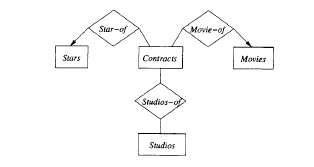
\includegraphics[width=0.7\linewidth]{images/worksheet_14_1.png}
    \end{center}

    accounts may be held jointly by several customers, we associate with each customer
    an "account set," and accounts are members of one or more account sets.
    Assuming the meaning of the various relationships and attributes are as expected
    given their names, criticize the design. What design rules are violated?
    Why? What modifications would you suggest?

    \bigskip

    \begin{center}
    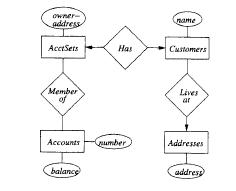
\includegraphics[width=0.7\linewidth]{images/worksheet_14_2.png}
    \end{center}

    \item \textbf{Exercise 4.2.2:} Under what circumstances (regarding the unseen attributes
    of Studios and Presidents) would you recommend combining the two entity sets
    and relationship in Fig. 4.3 into a single entity set and attributes?

    \item \textbf{Exercise 4.2.3:} Suppose we delete the attribute address from Studios in
    Fig. 4.7. Show how we could then replace an entity set by an attribute. Where
    would that attribute appear?

    \item \textbf{Exercise 4.2.4:} Give choices of attributes for the following entity sets in
    Fig. 4.13 that will allow the entity set to be replaced by an attribute:

    \bigskip

    Births, with four relationships, one between Births and each of the other entity
    sets, as suggested in Fig. 4.16. Use arrows (indicating that certain of these
    relationships are many-one) to represent the following conditions

    \bigskip

    \begin{enumerate}[a)]
        \item Every baby is the result of a unique birth, and every birth is of a unique baby.
        \item In addition to (a), every baby has a unique mother.
        \item In addition to (a) and (b), for every birth there is a unique doctora) Every baby is the result of a unique birth, and every birth is of a unique baby.
    \end{enumerate}

    \bigskip

    In each case, what design flaws do you see?

    \item \textbf{Exercise 4.4.1:} One way to represent students and the grades they get in
    courses is to use entity sets corresponding to students, to courses, and to "enrollments."
    Enrollment entities form a "connecting" entity set between students
    and courses and can be used to represent not only the fact that a student is
    taking a certain course, but the grade of the student in the course. Draw an
    E/R diagram for this situation, indicating weak entity sets and the keys for the
    entity sets. Is the grade part of the key for enrollments?

    \item \textbf{Exercise 4.4.2:} Modify your solution to Exercise 4.4.1 so that we can record
    grades of the student for each of several assignments within a course. Again,
    indicate weak entity sets and keys.

    \item \textbf{Exercise 4.4.3:} For your E/R diagrams of Exercise 4.2.6(a)~(c), indicate weak
    entity sets, supporting relationships, and keys.

    \item \textbf{Exercise 4.4.4:} Draw E/R diagrams for the following situations involving
    weak entity sets. In each case indicate keys for entity sets.

    \begin{enumerate}[a)]
        \item Entity sets Courses and Departments. A course is given by a unique department, but its only attribute is its number. Different departments can offer courses with the same number. Each department has a unique name.
        \item Entity sets Leagues, Teams, and Players. League names are unique. No league has two teams with the same name. No team has two players with the same number. However, there can be players with the same number on different teams, and there can be teams with the same name in different leagues.
    \end{enumerate}

    \item \textbf{Exercise 4.5.1:} Convert the E/R diagram of Fig. 4.29 to a relational database
    schema.

    \item \textbf{Exercise 4.5.2:} There is another E/R diagram that could describe the weak
    entity set Bookings in Fig. 4.29. Notice that a booking can be identified uniquely
    by the flight number, day of the flight, the row, and the seat; the customer is
    not then necessary to help identify the booking.

    \bigskip

    \begin{mdframed}
        \underline{\textbf{Relations with Subset Schema}}

        \bigskip

        You might imagine from Example 4.30 that whenever one relation R has a
        set of attributes that is a subset of the attributes of another relation S, we
        can eliminate R. That is not exactly true. R might hold information that
        doesn't appear inS because the additional attributes of S do not allow us
        to extend a tuple from R to S.

        \bigskip

        For instance, the Internal Revenue Service tries to maintain a relation
        People (name, ss\#) of potential taxpayers and their social-security numbers,
        even if the person had no income and did not file a tax return. They
        might also maintain a relation TaxPayers (name, ss\#, amount) indicating
        the amount of tax paid by each person who filed a return in the current
        year. The schema of People is a subset of the schema of TaxPayers, yet
        there may be value in remembering the social-security number of those
        who are mentioned in People but not in Taxpayers.

        \bigskip

        In fact, even identical sets of attributes may have different semantics,
        so it is not possible to merge their tuples. An example would be two
        relations Stars (name, addr) and Studios (name, addr). Although the
        schemas look alike, we cannot turn star tuples into studio tuples, or viceversa.
        On the other hand, when the two relations come from the weak-entityset
        construction, then there can be no such additional value to the relation
        with the smaller set of attributes. The reason is that the tuples of the
        relation that comes from the supporting relationship correspond one-forone
        with the tuples of the relation that comes from the weak entity set.
        Thus, we routinely eliminate the former relation.
    \end{mdframed}

    \bigskip

    \begin{enumerate}[a)]
        \item Revise the diagram of Fig. 4.29 to reflect this new viewpoint.
        \item Convert your diagram from (a) into relations. Do you get the same database schema as in Exercise 4.5.1?
    \end{enumerate}

    \item \textbf{Exercise 4.5.3:} The E/R diagram of Fig. 4.30 represents ships. Ships are said
    to be sisters if they were designed from the same plans. Convert this diagram
    to a relational database schema.

    \item \textbf{Exercise 4.5.4:} Convert the following E/R diagrams to relational database
    schemas.

    \begin{enumerate}[a)]
        \item Figure 4.22.
        \item Your answer to Exercise 4.4.1.
        \item Your answer to Exercise 4.4.4(a).
        \item Your answer to Exercise 4.4.4(b).
    \end{enumerate}

    \begin{center}
    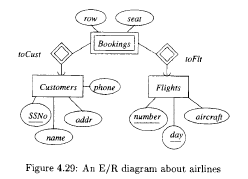
\includegraphics[width=0.7\linewidth]{images/worksheet_14_3.png}
    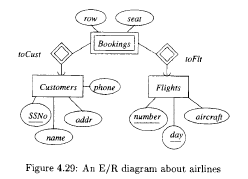
\includegraphics[width=0.7\linewidth]{images/worksheet_14_4.png}
    \end{center}


\end{enumerate}

\end{document}